\documentclass[11pt]{article}

\usepackage[margin=1.1in]{geometry}
\usepackage{amsmath,amssymb,amsthm}
\usepackage{mathpazo}
\usepackage{tikz}
\usetikzlibrary{arrows.meta,positioning,calc}
\usepackage{listings}
\usepackage{microtype}
\usepackage[colorlinks=true,linkcolor=blue!50!black,citecolor=blue!50!black,urlcolor=blue!50!black]{hyperref}

\theoremstyle{plain}
\newtheorem{theorem}{Theorem}
\newtheorem{proposition}[theorem]{Proposition}
\newtheorem{lemma}[theorem]{Lemma}
\newtheorem{corollary}[theorem]{Corollary}
\newtheorem{conjecture}[theorem]{Conjecture}

\theoremstyle{definition}
\newtheorem{definition}[theorem]{Definition}
\newtheorem{question}[theorem]{Question}

\theoremstyle{remark}
\newtheorem{remark}[theorem]{Remark}

\lstdefinestyle{rho}{
  basicstyle=\ttfamily\small,
  columns=fullflexible,
  keepspaces=true,
  showstringspaces=false,
  breaklines=true,
  frame=single,
  framesep=4pt,
  xleftmargin=2pt,
  commentstyle=\itshape\color{black!55},
  morecomment=[l]{//},
}
\lstset{style=rho}

\newcommand{\enc}[1]{[\![#1]\!]}
\newcommand{\Proc}{\mathbf{Proc}}
\newcommand{\NLS}{\mathbf{NLS}}
\newcommand{\Tang}{\mathbf{Tang}}

\title{The Point as Redex\\[2pt]
\large Finite Geometries as Reflective Higher-Order Processes}
\author{L. G. Meredith\\ \small F1R3FLY.io}
\date{July 2026}

\begin{document}
\maketitle

\begin{abstract}
A companion note rebuilds a 2005 encoding of knot diagrams as concurrent processes in
core rholang with cost accounting. The same 2005 investigation produced a second, much
shorter note: an encoding of the Fano plane in which \emph{lines are processes and points
are sets of redexes}. This note takes up that second encoding and argues that it is the
general recipe for Batten's axiomatic presentation of finite geometries. The organising
decision is the one named in the title. A point is not given a term; it is given no
inhabitant at all, and exists only as the set of communications the lines through it make
possible. We show that this decision has three consequences. First, it forces mixed
summation: at a point carrying $k \geq 3$ lines no orientation of the pairwise channels
can make every line's local offer homogeneous, so the calculus must be a variant of rho
with mixed choice, and we show this widens an existing former rather than adding a
constructor. Second, it identifies the knot encoding as the degenerate case: knot diagrams
are conflict-free because general position caps the multiplicity of an incidence at two,
and geometry is precisely the study of the coincidences that do not perturb away. Third,
it externalises the resolution of nondeterminism to a scheduler, leaving the strength of
that scheduler as a datum about the geometry rather than about the term. We give the
recipe, prove the well-definedness of its naming discipline from Batten's second axiom,
work the Fano plane, state the encoding functor and the faithfulness question, and close
with the questions this construction opens and does not answer.
\end{abstract}

\section{Introduction}

The original 2005 investigation \cite{Knots05} produced two notes. The first read a knot
diagram as a signalling network: a crossing is a gate, the over-strand passes a signal
through and opens a latch, the under-strand waits on that latch, and the arcs of the
diagram are the wires. That note has now been rebuilt in core rholang with cost
accounting \cite{KnotsNote}, where the Reidemeister moves become weak bisimulations, the
old demand for ``enough current'' becomes a liveness condition on a token ledger, and the
signed cost of one period is exactly twice the writhe.

The second note \cite{Fano05} was three pages long and did something different. It encoded
the Fano plane, and the encoding inverted the assignment: \emph{lines} became processes,
and \emph{points} became sets of redexes. Its closing observation was that the method was
not specific to the Fano plane but was read off the incidence structure. This note takes
that observation seriously and asks what it takes to make it a theorem about Batten's
presentation of finite geometry \cite{Batten}.

The step from the first note to the second is a step from topology to geometry, and it is
worth saying at the outset what makes it a real step rather than a change of example. A
knot diagram is a $4$-valent plane graph because a generic projection of a $1$-manifold
into the plane has only transverse double points; triple points are non-generic and can be
perturbed away by isotopy. Incidence geometry is the study of the coincidences one is
\emph{not} permitted to perturb. Desargues, Pappus and Fano are all assertions that
certain triples are forced to be collinear --- degeneracies a topologist removes and a
geometer keeps. We will see that this difference is not decorative: it is exactly the
difference between a conflict-free process and one with genuine races, and it is why the
geometric case needs more calculus than the topological one.

The organising decision is the one in the title. In the knot encoding the crossing --- a
point of the diagram --- is a process, the gate. In the Fano encoding a point is given no
term. It is an \emph{event site}: the set of communications the lines through it make
available, at most one of which occurs. That refusal to inhabit the point is what makes
the construction interesting, because it leaves the resolution of the resulting contention
to an external resource. What the geometry supplies is the shape of the contention; what
resolves it is a scheduler, and the strength of that scheduler is a separate datum. This
note develops the first half and deliberately leaves the second half open; see
Section~\ref{sec:outlook}.

\paragraph{What is in scope.} The encoding, its well-definedness, the calculus it requires,
the Fano plane worked in full, the relationship to the knot encoding, the standing (as
against one-shot) form of a geometry, and the statement of the functor and its
faithfulness question. Cost accounting is deliberately absent, for a reason given in
Section~\ref{sec:outlook}.

\section{Batten's presentation}
\label{sec:batten}

We follow \cite{Batten} closely, because the shape of that presentation is what the
hypothesis is about.

Batten works throughout with a set $P$ of \emph{points} and a set $L$ whose elements are
certain \emph{subsets} of $P$, called \emph{lines}. A \emph{space} is a pair $S = (P,L)$
subject to axioms. Note the normalisation already present: a line \emph{is} its set of
points, so there are no parallel edges and no line is determined by anything other than its
incidences.

\begin{definition}[Near-linear space]
A \emph{near-linear space} is a space $S = (P,L)$ such that
\begin{description}
\item[\textup{NL1}] any line has at least two points, and
\item[\textup{NL2}] two points are on at most one line.
\end{description}
\end{definition}

By NL2 the line on two distinct points, when it exists, is unique and is written $pq$. The
dual statement is immediate and will matter to us:

\begin{lemma}[{\cite[Lemma 1.2.1]{Batten}}]
\label{lem:meet}
Two distinct lines of a near-linear space intersect in at most one point.
\end{lemma}

Write $v = |P|$, $b = |L|$, $v(\ell)$ for the number of points on $\ell$, and $b(p)$ for
the number of lines on $p$.

Two constructions from \cite[\S1.3]{Batten} will be used. The \emph{dual space} of
$S = (P,L)$ has $L$ as its points, and as its lines the pencils --- the sets of at least
two lines of $S$ through a fixed point. Batten shows (Lemma 1.3.1) that the dual of a
near-linear space is a near-linear space. And, crucially for us:

\begin{definition}[{\cite[\S1.3]{Batten}}]
A \emph{graph} is a near-linear space in which every line has precisely two points.
\end{definition}

The spine of the whole book is a single number.

\begin{definition}[Connection number]
For a point $p$ not on a line $\ell$, the \emph{connection number} $c(p,\ell)$ is the
number of points of $\ell$ joined to $p$ by a line.
\end{definition}

Batten's chapters are then a stratification by $c$: near-linear spaces place no constraint
on it; linear spaces demand $c(p,\ell) = v(\ell)$ always; projective and affine spaces are
special cases of these; polar spaces demand $c(p,\ell) \in \{1, v(\ell)\}$; generalized
quadrangles demand $c(p,\ell) = 1$; partial geometries demand $c(p,\ell) = \alpha$ for a
fixed positive integer $\alpha$. Seven chapters, one observable, five constraints on it.
Finally, \cite[\S1.7]{Batten} introduces \emph{linear functions}, which is where Batten
pins down when two spaces are to be regarded as the same; these are the morphisms of the
source category in Section~\ref{sec:functor}.

We will use as running example Batten's own first appearance of the Fano plane
\cite[Example 1.1.2]{Batten}: seven points, seven lines, three points on each line and
three lines on each point, with points labelled $0,\dots,6$ and lines the seven sets
$\{1+i,\,2+i,\,4+i\}$ for $0 \le i \le 6$, read modulo $7$. Explicitly, and fixing names
for the rest of this note,
\[
\begin{array}{llll}
M_1 = \{1,2,4\}, & M_2 = \{2,3,5\}, & M_3 = \{3,4,6\}, & M_4 = \{0,4,5\},\\
M_5 = \{1,5,6\}, & M_6 = \{0,2,6\}, & M_7 = \{0,1,3\}. &
\end{array}
\]

\begin{figure}[t]
\centering
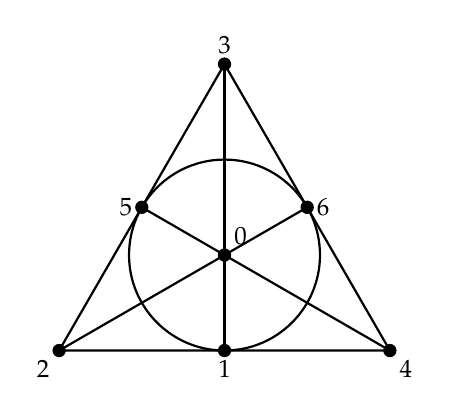
\begin{tikzpicture}[scale=1.05,
  pt/.style={circle,fill=black,inner sep=1.7pt},
  lbl/.style={font=\small}]
  \coordinate (v2) at (0,0);
  \coordinate (v4) at (4,0);
  \coordinate (v3) at (2,3.4641);
  \coordinate (m1) at (2,0);
  \coordinate (m5) at (1,1.7321);
  \coordinate (m6) at (3,1.7321);
  \coordinate (c0) at (2,1.1547);

  \draw[thick] (v2) -- (v4) -- (v3) -- cycle;
  \draw[thick] (v2) -- (m6);
  \draw[thick] (v4) -- (m5);
  \draw[thick] (v3) -- (m1);
  \draw[thick] (c0) circle (1.1547);

  \node[pt] at (v2) {}; \node[lbl,below left]  at (v2) {$2$};
  \node[pt] at (v4) {}; \node[lbl,below right] at (v4) {$4$};
  \node[pt] at (v3) {}; \node[lbl,above]       at (v3) {$3$};
  \node[pt] at (m1) {}; \node[lbl,below]       at (m1) {$1$};
  \node[pt] at (m5) {}; \node[lbl,left]        at (m5) {$5$};
  \node[pt] at (m6) {}; \node[lbl,right]       at (m6) {$6$};
  \node[pt] at (c0) {}; \node[lbl,above right] at (c0) {$0$};
\end{tikzpicture}
\caption{The Fano plane in Batten's labelling. The three sides carry
$M_1 = \{1,2,4\}$, $M_2 = \{2,3,5\}$, $M_3 = \{3,4,6\}$; the three medians carry
$M_4 = \{0,4,5\}$, $M_6 = \{0,2,6\}$, $M_7 = \{0,1,3\}$; the circle carries
$M_5 = \{1,5,6\}$. Every point lies on three lines and every line carries three points,
so under the encoding of Section~\ref{sec:recipe} every one of the seven points is a
three-way contention.}
\label{fig:fano}
\end{figure}

\section{The recipe}
\label{sec:recipe}

We extract the scheme from \cite{Fano05}. It has four parts.

\begin{enumerate}
\item \textbf{Lines are processes.} The geometry is the parallel composition of its lines,
$\enc{S} = \prod_{\ell \in L} \enc{\ell}$.
\item \textbf{Points are not terms.} A point is a set of redexes: the communications
available among the lines through it.
\item \textbf{A line is a parallel composition of one component per incident point}, and
each such component is a \emph{sum} with one summand per other line through that point.
So a line's business at a point is to choose which of its co-incident lines it meets there.
\item \textbf{Channels are named by pairs of lines.} For lines $\ell_i \neq \ell_j$ we
write $x_{ij}$ for the channel at their common point, oriented so that $\ell_i$ receives
and $\ell_j$ sends.
\end{enumerate}

The continuations are left as unknowns: $\ell_i$ receiving on $x_{ij}$ continues as
$P_{ij}$, and $\ell_j$ sending carries a payload $Q_{ij}$. The skeleton is the incidence
data alone.

The fourth part is the one that needs justifying, and the justification is Batten's second
axiom.

\begin{proposition}[NL2 is the well-definedness condition]
\label{prop:naming}
The naming discipline of part \textup{4} is well defined --- that is, an unordered pair of
distinct lines determines at most one channel, and hence at most one point --- if and only
if any two distinct lines meet in at most one point. In a space satisfying \textup{NL2},
this holds by Lemma~\ref{lem:meet}.
\end{proposition}

\begin{proof}
Immediate from the definition: the channel $x_{ij}$ is indexed by the pair $\{i,j\}$, so
the scheme assigns a unique channel to a pair exactly when the pair has a unique
intersection point to assign it to.
\end{proof}

This is worth pausing on. The base axiom system is not something the encoding must
\emph{enforce}; it is the precondition for the encoding to be definable at all. Similarly
NL1, that a line has at least two points, is what makes $\enc{\ell}$ a nontrivial parallel
composition rather than a single component. A near-linear space is not one kind of thing
this recipe can encode; it is the exact class of things the recipe applies to.

\begin{remark}[Counting]
For a space in which every point lies on $k$ lines, each point contributes $\binom{k}{2}$
channels and $2\binom{k}{2}$ prefixes, one endpoint per line involved. For the Fano plane,
$7 \cdot \binom{3}{2} = 21$ channels and $42$ prefixes, distributed as $7$ lines $\times$
$3$ components $\times$ $2$ summands.
\end{remark}

\section{Mixed summation is forced}
\label{sec:mixed}

The calculus of \cite{Fano05} is a version of the $\pi$-calculus with guarded summation,
and the sums it writes are \emph{mixed}: input and output summands occur in the same
choice. Core rholang, as used in \cite{KnotsNote}, has neither output prefixing nor mixed
sums. Its receipt is already a choice --- a \texttt{;}-separated list of
\texttt{\&}-joined groups --- but an input-only one. The question is whether the mixing is
essential or an artefact of how the 2005 note happened to orient its channels. It is
essential, and the reason is a two-line argument about tournaments.

Fix a point $p$ lying on $k$ lines. The channels at $p$ are indexed by the pairs from those
$k$ lines, so they form the edge set of the complete graph $K_k$; an assignment of
directions to all of them is a tournament on $K_k$. Call a line's component at $p$
\emph{homogeneous} if all its summands are receives, or all are sends.

\begin{proposition}[Orientation obstruction]
\label{prop:tournament}
There is an orientation of the channels at $p$ making every incident line's component
homogeneous if and only if $k \leq 2$.
\end{proposition}

\begin{proof}
A line's component at $p$ is homogeneous exactly when the corresponding vertex of $K_k$ is
a source or a sink of the tournament. Suppose every vertex is a source or a sink, and
partition the vertices accordingly. Two sources cannot be adjacent, since the edge between
them must be directed and would give one of them an in-edge; likewise two sinks. As $K_k$
is complete, each class therefore contains at most one vertex, so $k \leq 2$. Conversely
$K_1$ has no edges and $K_2$ has one, which may be directed either way.
\end{proof}

\begin{corollary}
\label{cor:mixed}
Under the recipe of Section~\ref{sec:recipe}, any near-linear space with a point on three
or more lines requires mixed summation. In particular every point of a projective plane of
order $n \geq 2$ requires it, since $b(p) = n+1 \geq 3$.
\end{corollary}

\begin{figure}[t]
\centering
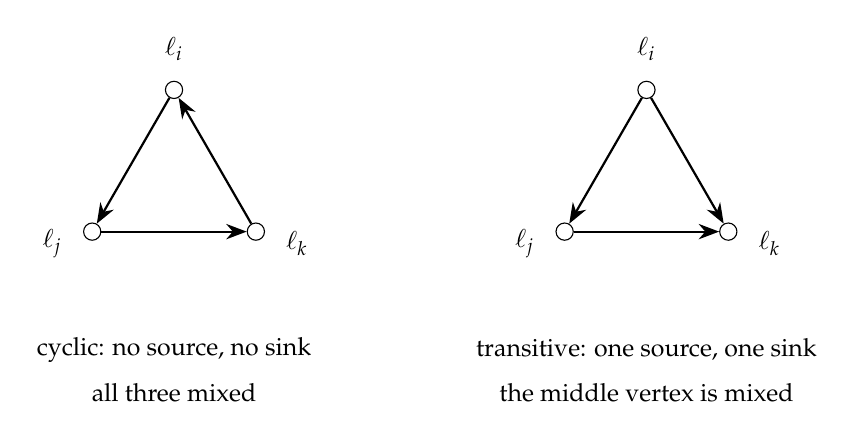
\begin{tikzpicture}[scale=1.0,
  pt/.style={circle,draw,fill=white,inner sep=2.2pt},
  ar/.style={-{Stealth[length=2.6mm]},thick}]

  \begin{scope}
    \node[pt] (a) at (90:1.2)  {}; \node[font=\small,above] at (90:1.45) {$\ell_i$};
    \node[pt] (b) at (210:1.2) {}; \node[font=\small,left]  at (210:1.5) {$\ell_j$};
    \node[pt] (c) at (330:1.2) {}; \node[font=\small,right] at (330:1.5) {$\ell_k$};
    \draw[ar] (a) -- (b);
    \draw[ar] (b) -- (c);
    \draw[ar] (c) -- (a);
    \node[font=\small] at (0,-2.1) {cyclic: no source, no sink};
    \node[font=\small] at (0,-2.65) {all three mixed};
  \end{scope}

  \begin{scope}[xshift=6cm]
    \node[pt] (a) at (90:1.2)  {}; \node[font=\small,above] at (90:1.45) {$\ell_i$};
    \node[pt] (b) at (210:1.2) {}; \node[font=\small,left]  at (210:1.5) {$\ell_j$};
    \node[pt] (c) at (330:1.2) {}; \node[font=\small,right] at (330:1.5) {$\ell_k$};
    \draw[ar] (a) -- (b);
    \draw[ar] (a) -- (c);
    \draw[ar] (b) -- (c);
    \node[font=\small] at (0,-2.1) {transitive: one source, one sink};
    \node[font=\small] at (0,-2.65) {the middle vertex is mixed};
  \end{scope}
\end{tikzpicture}
\caption{The two tournaments on three lines through a point, up to relabelling
(Proposition~\ref{prop:tournament}). Neither makes all three components homogeneous, and
there is nothing else to try. An arrow $\ell \to \ell'$ means $\ell$ sends and $\ell'$
receives on their shared channel.}
\label{fig:tournament}
\end{figure}

\subsection{The variant}

What is needed is smaller than it might appear, and the 2005 notation already says so: its
input summands are prefixes with continuations, $x?(y)P$, while its output summands are
bare sends, $x!(Q)$, with nothing trailing. So output prefixing is not required and
synchrony is not required. The only new dynamics is \emph{commitment}: firing one summand
discards its alternatives.

\begin{definition}[Core rholang with mixed summation]
\label{def:variant}
Let $\rho^{+}$ be generated by
\[
P,Q ::= 0 \;\mid\; \textstyle\sum_{i} \alpha_i \;\mid\; P \mid Q \;\mid\;
\mathsf{new}\ x\ \mathsf{in}\ \{P\} \;\mid\; {*}x \;\mid\;
\mathsf{def}\ X(\vec y) = P \;\mid\; X(\vec z),
\]
where each summand $\alpha_i$ is either an asynchronous send $x!(Q)$ or a receipt
$\mathsf{for}(\vec y_1 \leftarrow \vec z_1\ \&\ \cdots)\{P\}$, with quoting $@P$ and
dereferencing ${*}x$ realising reflection as usual. Communication is as in core rholang,
with the additional rule that when a summand of a sum fires, the whole sum is consumed.
\end{definition}

Three observations about this definition, in decreasing order of comfort.

\begin{remark}[It widens a former rather than adding one]
Rholang's receipt is already a choice construct: the \texttt{;}-separated list of
\texttt{\&}-joined groups. Definition~\ref{def:variant} widens the grammar of its summands
to admit sends; it does not introduce a new term former. This matters for the discipline
of \cite[Remark 1]{KnotsNote}, where $\mathsf{def}$ was insisted to be derived rather than
primitive on the ground that the structural connectives of a logic generated from a theory
are read off that theory's constructors, so a new constructor puts a new connective into
the vocabulary of any generated classifier. Here the connective is already in the
vocabulary; what changes are the transition rules and the class of inhabitants. The change
is lighter, not free.
\end{remark}

\begin{remark}[What must still be settled]
The equational status of $\sum$ --- presumably a commutative monoid with $0$ --- is not
a formality in a reflective calculus, because name equality is decided on
structural-congruence classes. Admitting sums into the equational theory is therefore a
question for an implementation as much as for a semantics, and this note does not settle
it.
\end{remark}

\begin{remark}[Expressiveness is genuinely increased]
Mixed choice is not encodable into the separate-choice or asynchronous fragments by a
uniform, distribution-preserving encoding; this is the substance of Palamidessi's
separation results for the $\pi$-calculus. So $\rho^{+}$ is a strictly richer theory than
core rholang, and any faithfulness claim below is a claim relative to $\rho^{+}$. The
honest framing is that $\rho^{+}$ is another object of the category of graph-structured
lambda theories, related to core rholang by a bisimulation-preserving map in one direction
only, and that the encoding of a geometry lands in it.
\end{remark}

\section{The Fano plane, worked}
\label{sec:worked}

Fix the transitive orientation at every point: at a point on lines $M_i, M_j, M_k$ with
$i<j<k$, direct each channel from the higher index to the lower, so that $x_{ij}$ is
received by $M_i$ and sent by $M_j$. By Proposition~\ref{prop:tournament} this makes the
least-indexed line at each point all-receiving, the greatest all-sending, and the middle
one mixed.

The pencils of the Fano plane in Batten's labelling are
\[
\begin{array}{llll}
p_0:\ \{M_4,M_6,M_7\}, & p_1:\ \{M_1,M_5,M_7\}, & p_2:\ \{M_1,M_2,M_6\}, & p_3:\ \{M_2,M_3,M_7\},\\
p_4:\ \{M_1,M_3,M_4\}, & p_5:\ \{M_2,M_4,M_5\}, & p_6:\ \{M_3,M_5,M_6\}. &
\end{array}
\]

Take $M_4 = \{0,4,5\}$, which meets all three cases. At $p_0$ its pencil-mates are
$M_6, M_7$ and $M_4$ is least, so its component is all-receiving. At $p_4$ its mates are
$M_1, M_3$ and $M_4$ is greatest, so its component is all-sending. At $p_5$ its mates are
$M_2, M_5$ and $M_4$ is in the middle: it sends on $x_{24}$ and receives on $x_{45}$. Hence

\[
\begin{aligned}
\enc{M_4} \;=\;
&\underbrace{\big(\,\mathsf{for}(y \leftarrow x_{46})\{P_{46}\} \;+\;
                  \mathsf{for}(y \leftarrow x_{47})\{P_{47}\}\,\big)}_{\text{at } p_0
                  \text{: all-receiving}}\\[2pt]
\Big|\;\;
&\underbrace{\big(\, x_{14}!(Q_{14}) \;+\; x_{34}!(Q_{34}) \,\big)}_{\text{at } p_4
                  \text{: all-sending}}\\[2pt]
\Big|\;\;
&\underbrace{\big(\, x_{24}!(Q_{24}) \;+\;
                  \mathsf{for}(y \leftarrow x_{45})\{P_{45}\} \,\big)}_{\text{at } p_5
                  \text{: mixed}}
\end{aligned}
\]

and the plane is
\[
\enc{\mathrm{Fano}} \;=\; \mathsf{new}\ x_{12},\dots,x_{67}\ \mathsf{in}\
\{\, \enc{M_1} \mid \enc{M_2} \mid \enc{M_3} \mid \enc{M_4} \mid \enc{M_5} \mid
\enc{M_6} \mid \enc{M_7} \,\}
\]
if one wishes to close it, or with the $x_{ij}$ left free if one wishes to observe it ---
a distinction that will matter in Section~\ref{sec:functor}. The third component of
$\enc{M_4}$ is a mixed sum, and by Corollary~\ref{cor:mixed} no relabelling removes it.

Note what the sums are doing. At $p_5$ the lines $M_2, M_4, M_5$ each offer two branches,
and the three available redexes are $M_2$-with-$M_4$, $M_2$-with-$M_5$, and
$M_4$-with-$M_5$. Exactly one of them can occur, because whichever fires consumes the
whole sum on both sides. The point is a three-way race, and the geometry has said nothing
about which way it goes.

\section{Knots as the degenerate case}
\label{sec:knots}

The knot encoding of \cite{KnotsNote} makes the opposite assignment: the point of the
diagram --- the crossing --- is a process, the gate, and the lines of the diagram --- the
arcs --- are channels. Proposition~1 of that note establishes that every arc occurs
exactly once as an output port and exactly once as an input port. In net-theoretic terms
that is precisely \emph{conflict-freedom}: the encoding is a marked graph, which is why
liveness, conservation and periodicity come as cheaply as they do there, and why the
minimal-live-current question reduces to a circuit-covering problem solvable in
polynomial time.

The natural suspicion is that the geometric case could be pushed back into that class by
choosing the other assignment. It cannot, and the reason is a degree condition that is
insensitive to which assignment one picks.

\begin{proposition}[Where conflict lives]
\label{prop:conflict}
Let $S = (P,L)$ be a near-linear space.
\begin{enumerate}
\item Under the \emph{points-as-processes} assignment, in which each line is a channel
shared by its incident points, a conflict site is a line with three or more points. The
encoding is conflict-free if and only if $S$ is a graph in Batten's sense.
\item Under the \emph{lines-as-processes} assignment of Section~\ref{sec:recipe}, a
conflict site is a point on three or more lines. The encoding is conflict-free if and
only if the dual space of $S$ is a graph, i.e.\ $b(p) \leq 2$ for every point.
\end{enumerate}
\end{proposition}

\begin{proof}
In either case a communication is binary, so a channel with $m$ participants admits
$\binom{m}{2}$ competing pairings and is conflict-free exactly when $m \leq 2$. In case 1
the participants at a line $\ell$ are its points, so $m = v(\ell)$, and $v(\ell) = 2$ for
all $\ell$ is the definition of a graph. In case 2 the participants at a point $p$ are the
lines through it, so $m = b(p)$, and this is the same condition on the dual space.
\end{proof}

\begin{corollary}
A knot diagram, read with crossings as points and arcs as lines, lies on the good side of
case \textup{1}: an arc joins exactly two crossings, so $v(\ell) = 2$ throughout. A
projective plane of order $n \geq 2$ lies on the bad side of both, since $v(\ell) = b(p) =
n+1 \geq 3$ and the plane is self-dual.
\end{corollary}

So the expressiveness jump between the two 2005 notes is not an artefact of the
dualisation. It is the passage out of Batten's graph case, and it is dualisation-invariant.

\begin{remark}[Chirality is the orientation of $K_2$]
Proposition~\ref{prop:tournament} for $k=2$ says that the single channel at a degree-two
site may be oriented either way, freely. In the knot encoding that free bit is exactly
chirality: which strand produces the latch and which joins on it. Mixed choice is
therefore not a new phenomenon introduced by geometry but what chirality becomes when a
point carries more than two lines and the free bit can no longer be chosen consistently.
\end{remark}

\begin{remark}[The reason the cap is there]
It is worth naming why knot diagrams satisfy $v(\ell) = 2$. It is general position: a
generic projection of a $1$-manifold has transverse double points and no triple points,
and any triple point that appears may be perturbed away. So the conflict-freedom of the
knot encoding is a consequence of a theorem of topology, not of a modelling convention.
Geometry is what is left when perturbation is disallowed, and conflict is what that looks
like in a process calculus.
\end{remark}

\begin{remark}[A caveat about the analogy]
A knot diagram read as an incidence structure is a $4$-regular plane \emph{multigraph} and
not a near-linear space: two crossings of the standard trefoil diagram are joined by two
distinct arcs, so NL2 fails. Proposition~\ref{prop:conflict} is therefore a statement about
the two encodings and the degree conditions they are sensitive to, not a claim that knot
diagrams are objects of Batten's category. Making the comparison literal would require
either a multi-line-tolerant weakening of NL2 or a subdivision of the diagram, and we do
not pursue either here.
\end{remark}

\begin{remark}[Proof-irrelevance]
There is a second reading of Proposition~\ref{prop:conflict} worth recording. A
conflict-free network is confluent, so every schedule of it produces the same result up to
the equivalence of interest; the resolution carries no observable information. The knot
encoding is thus \emph{proof-irrelevant} throughout in the sense of \cite{Choice}: it has
no scheduler-side content anywhere. Under the recipe of Section~\ref{sec:recipe} a
geometry is the opposite extreme --- an object every one of whose points is a nontrivial
race. This is the precise sense in which the point-as-redex decision buys something.
\end{remark}

\section{Standing geometries}
\label{sec:standing}

The skeleton of Section~\ref{sec:recipe} has a defect that \cite{Fano05} names and does
not fix, and it is the same defect \cite{KnotsNote} spends its third section repairing.
Every summand is linear, so it is spent by its own firing; the encoded geometry is a
one-shot cell that evaporates after one passage. Such a term models a traversal of a
geometry rather than the geometry, and --- decisively, given that the note's headline
observation is that geometries compose by parallel composition --- a geometry built from
one-shot components cannot be composed and reused.

The fix is the one \cite{Fano05} itself gestures at, with the hint
\[
x?(y)\big({*}y \mid x!(y)\big) \;\big|\; x!\big(x?(y)({*}y \mid x!(y)) \mid P\big)
\;\longrightarrow^{*}\; P \mid P \mid P \mid \cdots
\]
which is recursion from reflection: quote the body, pass the quotation to itself, drop it
at each unfolding. This is exactly the mechanism of \cite[Remark 1]{KnotsNote}, where it is
also observed that unfolding is an equation rather than a rewrite and so is never charged
by a cost semantics.

The placement question that \cite{KnotsNote} had to answer --- where in the gate the
reinstatement goes --- has a simpler answer here, because the sum makes the event
unambiguous. Firing at a point consumes exactly one component of each of the two lines
involved, and nothing else. So each line reinstates its own component at that point:

\begin{lstlisting}
def At_i_p(...) = {
    x_ij!( Q_ij ) + for (y <- x_ik) { P_ik | At_i_p(...) }
}
\end{lstlisting}

with the reinstatement in each continuation of the sum. One point-event releases exactly
two copies, one per participating line, which is correct: the components belong to
different lines and each must be restored independently. Nothing else at the point is
touched, so the other line through $p$ still offers both its branches, now against a
freshly armed pair.

This gives the taxonomy that \cite{Fano05} sets out in its discussion, which we record
because Section~\ref{sec:outlook} returns to it:

\begin{description}
\item[Grade 0] the bare skeleton: incidence data as a pattern of redexes, spent by one
passage.
\item[Grade 1] a \emph{standing} geometry: solve for $P_{ij}, Q_{ij}$ so that the space
reproduces itself, giving a stable geometry that survives being used.
\item[Grade 2] an \emph{evolving} geometry: solve for $P_{ij}, Q_{ij}$ so that as lines
interact the space becomes a different geometry.
\end{description}

\begin{remark}[The grades are a term-side ladder]
It is tempting to read the three grades as a ladder of increasing demands on the
resolution of nondeterminism, with grade~2 requiring dependent choice because later
contentions depend on earlier selections. That reading is wrong, and it is worth saying
so explicitly because it collapses a distinction the surrounding programme rests on
\cite[Principle 1]{Choice}: the confluent communication skeleton and the resolution of
races are orthogonal axes. Evolving geometry can be programmed entirely in term structure
--- the continuation computes the successor space, deterministically, given whatever the
point handed it --- with the choice structure unchanged. The grades move on the term axis.
What moves on the choice axis is discussed in Section~\ref{sec:outlook}.
\end{remark}

\section{The encoding functor, and what faithfulness would mean}
\label{sec:functor}

We state the target and the open question; we do not prove the theorem here.

Let $\NLS$ be the category whose objects are near-linear spaces and whose morphisms are
Batten's linear functions \cite[\S1.7]{Batten} --- or, for a first pass, its isomorphisms,
which is where Batten pins down when two spaces are the same. Let $\Proc_{\sim}$ be
$\rho^{+}$ processes with free boundary modulo context-labelled bisimulation, in the sense
of the relative-expressiveness apparatus: bisimulation is taken over transitions labelled
by contexts, the encoding maps contexts as well as terms, and the observing contexts are
restricted to the image of the geometry contexts rather than ranging over all of
$\rho^{+}$.

\begin{definition}
$\enc{-} : \NLS \to \Proc_{\sim}$ sends a near-linear space to the parallel composition of
its line-processes with the channels $x_{ij}$ left free, and a linear function to the
induced renaming of channels.
\end{definition}

Leaving the $x_{ij}$ free is not incidental. In \cite[\S10]{KnotsNote} the corresponding
construction has to close the boundary --- a knot is a closed curve --- which makes every
step internal and leaves a live, periodic $\tau$-network that is nearly featureless as an
observable object, so that the weak-bisimulation class of a closed knot encoding cannot be
expected to carry knot type on its own. The geometric case does not have this problem. A
geometry has no closure step; its points are its observables, and they stay observable.

\begin{question}[Faithfulness]
\label{q:faithful}
Does $\enc{-}$ reflect as well as preserve the context-labelled transition structure? That
is, does no branching present in $\NLS$ survive into the image only in collapsed form?
\end{question}

This is the \emph{hosting} condition on $\enc{-}$, and it is the same question that stands
open for the knot encoding. Two reasons to think the geometric case is the more tractable
test. First, the boundary never closes, so the observables are not destroyed. Second, by
Remark~\ref{rem:branching} below, the image has genuine branching to observe.

\begin{remark}
\label{rem:branching}
By Proposition~\ref{prop:conflict}, $\enc{S}$ is conflict-free exactly when the dual of $S$
is a graph. Away from that degenerate case the transition system has real branching, and a
branching-time equivalence has something to distinguish. The knot encoding, being
conflict-free, is nearly confluent, so its bisimulation and trace theories nearly coincide
--- which is another face of the featurelessness complaint above. If one wants to
demonstrate a spatial-behavioural classifier, geometry may be the better first case
rather than the sequel.
\end{remark}

Beyond isomorphism, the substantive form of the hypothesis concerns the axioms rather than
the objects. Batten's stratification is by a single number, and one would like that number
to be legible in the process.

\begin{conjecture}[The connection number is a behavioural observable]
\label{conj:c}
There is a formula $\chi_{c=\kappa}$ in the spatial-behavioural logic generated from
$\rho^{+}$ such that $\enc{S} \models \chi_{c=\kappa}$ if and only if $c(p,\ell) = \kappa$
for all $p \notin \ell$ in $S$; and consequently Batten's classes --- linear spaces, polar
spaces, generalized quadrangles, partial geometries --- are the extensions in
$\Proc_{\sim}$ of five formulae over one observable.
\end{conjecture}

If this holds, then \cite[\S1.1]{Batten}, which opens the book with the consistency and
independence of axiom systems, acquires a computational reading: consistency of a system
is inhabitation of the corresponding type, and independence is non-derivability in the
generated logic. That is the cash value of the 2005 note's remark that the skeleton is
closer to a spatial-behavioural type than to a process.

\section{Outlook}
\label{sec:outlook}

The construction above settles the shape of the encoding and leaves several things open on
purpose. We list them with an indication of how far each is from being a computation
rather than a hope.

\paragraph{Choice is externalised, and finite geometry does not climb.} The point-as-redex
decision hands the resolution of every contention to a scheduler. In the framework of
\cite{Choice}, each point is an aperture whose choice-type is a $\forall\exists$: for the
contended slot, an admissible pairing exists. It should be said plainly that in Batten's
setting this type is trivial. Every fibre is a finite pencil, presented as a bag of
prefixes at a channel by construction; the index set is finite; the section is definable
outright, at the base of the stalk. Finite geometry is the \emph{calibration} regime: the
place to test a term assignment where one already knows the answer. What climbs the
strength order is cardinality and effectivity of the incidence structure --- infinite point
sets, infinite pencils, non-enumerable pencils --- and all three are outside Batten by
definition. The value of the recipe to the choice programme is that it is a uniform way of
turning an incidence structure into a contention structure, after which the cardinality
dials are there to turn.

\paragraph{The collaboration between choice and structure.} The two axes are orthogonal as
typing disciplines and coupled in their effect. A grade-2 term lays out a tree of possible
successor geometries; the scheduler plays that tree. This is the selection-function
picture of \cite{Choice} with the game tree supplied explicitly, which is usually the
missing ingredient. It also relocates the invariant: a dancing geometry has no single
space to point at, and the natural object is the trajectory system --- geometries as
states, transitions labelled by which pairing fired at which point --- with bisimulation
on that. Whether one wants the dance confluent, so that all fair trajectories converge and
the reached geometry is an invariant of the term, is a genuine fork and not a
choice-strength question.

\paragraph{Safety, liveness, and fairness.} Under the dance, Batten's axioms split. ``Is a
near-linear space'' is a safety property, true along every trajectory with no assumption
on the scheduler. ``Becomes a projective plane'', ``attains connection number $\alpha$
everywhere'', ``acquires a parallel class'' are liveness properties, true only under a
fairness discipline. We expect \emph{strong} fairness to be required rather than weak: a
branch at a point is enabled only when its partner currently offers the matching branch,
so enablement is intermittent and the continuously-enabled criterion does not reach it.
This is the geometric successor to the minimal-current analysis of \cite[\S5]{KnotsNote},
and it is a fairness discipline rather than a combinatorial optimum.

\paragraph{A computation to do first.} A step of a standing geometry selects, at each point
it touches, one pair from the pencil there, with a line free to fire at several of its
points at once since its components are in parallel. Fairness over an infinite run demands
that each of the $\binom{b(p)}{2}$ pairings at each point fire infinitely often. That is a
round-decomposition question about the design, and finite geometry already has the
vocabulary --- parallel classes, resolvability. The concrete first question is the period
structure of fair schedules of $\enc{\mathrm{Fano}}$, which is small enough to enumerate.

\paragraph{Symmetry breaking.} A finite geometry has a large automorphism group;
$\mathrm{PGL}(3,2)$, of order $168$, for the Fano plane. A fair schedule cannot respect it:
to serialise a symmetric contention the scheduler must pick, and picking breaks the
symmetry. Whether a fair schedule of a symmetric design is forced into a period that is a
proper multiple of anything intrinsic to the design is a sharp, finite question, and it is
the honest version of an analogy to discrete time crystals. We flag the analogy carefully:
a discrete time crystal is a \emph{driven} system whose response spontaneously locks to a
multiple of the drive period, breaking discrete time-translation symmetry, and the
equilibrium version is excluded by no-go results. A conservative marked graph with a
periodic orbit, such as the knot encoding, is a clock and not a crystal. What the geometric
case adds is a candidate for the missing ingredient: the scheduler as the drive, and as the
thing that breaks the symmetry.

\paragraph{Resource-constrained geometry.} Cost accounting is absent from this note by
design, and the reason is structural rather than editorial. The knot encoding is
\emph{conservative}: arc tokens are neither created nor destroyed, latches are created and
destroyed in matched pairs, and the orbit closes. Nothing in it degrades, because nothing
is lost. To study a geometry as a material --- structure that must be maintained, that
rusts --- one has to give up that conservation law, and the conservation law is exactly
what makes a diagram an invariant. \emph{Conservation is what makes a diagram an invariant;
loss is what makes a geometry a material.} That is a different note, and it connects to the
existing treatment of cost accounting as mortal computation and of the history endofunctor's
erasure lattice rather than to anything here. One asymmetry can be recorded now: the
\emph{signed} ledger of \cite{KnotsNote} is unlikely to transfer, because the sign there is
intrinsic --- the crossing sign, fixed by the orientation the DT traversal supplies ---
whereas the send/receive polarity of Section~\ref{sec:worked} is a gauge choice, not data.
We would expect solvency and liveness to carry over and the writhe-analogue to have no
counterpart, so that a geometric ledger measures upkeep rather than framing.

\paragraph{An artefact this note does not ship.} The companion \cite{KnotsNote} ships a
runnable term, and much of its credibility rests on that. $\rho^{+}$ is not implemented in
\texttt{f1r3node-rust}, so a generated Fano term has no interpreter today. The honest
remedy is a small reference reducer for Definition~\ref{def:variant} alongside a generator
from an incidence structure to a $\rho^{+}$ term, which would turn ``we posit a variant''
into ``here is the variant, and here is a geometry running in it''. Until then
Section~\ref{sec:mixed} is a promissory note in a paper whose companion cashed all of its,
and we mark it as such rather than leave the reader to notice.

\begin{thebibliography}{9}

\bibitem{Batten} L. M. Batten. \emph{Combinatorics of Finite Geometries}. Cambridge
University Press, 1st ed.\ 1986, 2nd ed.\ 1997.

\bibitem{Choice} L. G. Meredith. \emph{From the Axiom of Choice to Fair Scheduling: toward
a Curry--Howard correspondence for nondeterminism}. F1R3FLY.io research note, June 2026.

\bibitem{Fano05} L. G. Meredith. \emph{A $\pi$-calculus model of the Fano plane} (working
note, 2005).

\bibitem{Knots05} L. G. Meredith. \emph{Knots as processes} (working notes, 2005).

\bibitem{KnotsNote} L. G. Meredith. \emph{Knots as Cost-Accounted Rholang Processes: a
Dowker--Thistlethwaite-driven encoding and weak-bisimulation invariance}. F1R3FLY.io,
July 2026.

\bibitem{Node} F1R3FLY.io. \texttt{f1r3node-rust}: a pure-Rust F1R3FLY node with a rholang
interpreter. \url{https://github.com/F1R3FLY-io/f1r3node-rust}.

\bibitem{Commoner} F. Commoner, A. W. Holt, S. Even, and A. Pnueli. Marked directed graphs.
\emph{J. Comput. System Sci.} 5 (1971), 511--523.

\bibitem{Pala} C. Palamidessi. Comparing the expressive power of the synchronous and
asynchronous $\pi$-calculi. \emph{Math. Structures Comput. Sci.} 13(5) (2003), 685--719.

\bibitem{EO} M. H. Escard\'o and P. Oliva. Selection functions, bar recursion and backward
induction. \emph{Math. Structures Comput. Sci.} 20(2) (2010), 127--168.

\bibitem{Mer05} L. G. Meredith and M. Radestock. A reflective higher-order calculus.
\emph{Electr. Notes Theor. Comput. Sci.} 141(5) (2005), 49--67.

\end{thebibliography}

\end{document}
